\documentclass[../../main.tex]{subfiles}
\begin{document}
Decoder only transformers make up the base of generative pre-trained transformers (GPT).

\begin{figure}[t]
	\centering
	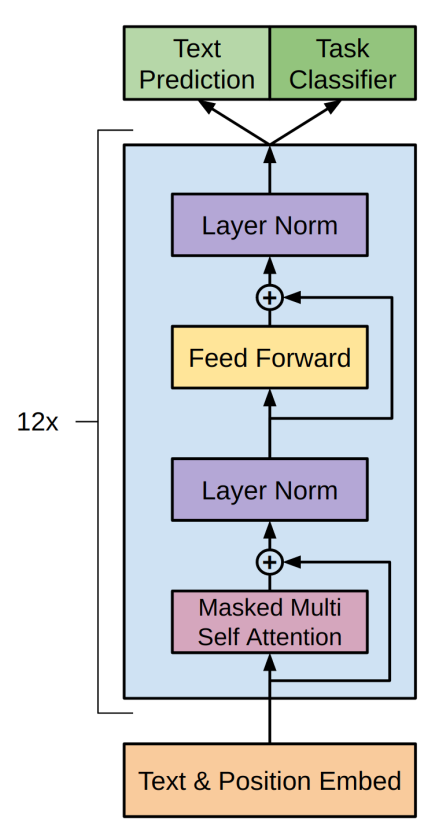
\includegraphics[scale=0.3]{include/images/gpt_architecture.png}
	\caption{The GPT archictuecture \cite{Radford2018}}
	\label{fig:gpt_arch}
\end{figure}

The GPT archtecture is shown in figure \ref{fig:gpt_arch}.
Training GPT happends in two phases, unsupervised pre-training and supervised finetuning.

In the unsupervised pre-training phase the models is training on unlabeled text data similiar to the pre-training of full transformer models.
They are trained to predict the next token for a input sequence of tokens.

Newer research on generation models focuses on scaling the network.
The \textit{scaling law} says that by simply increasing the amount of parameters of the network, the model capabilites increase.
Furthermore, at some scaling points the learning of emerging abilities happen, the model learns things it had not seens direclty in the training data.

As large language model scaling has reached billion parameter counts, only very few companies have the hardware to train or even run inference tasks.
\end{document}